\documentclass[12pt,a4paper]{article}
\usepackage[T2A]{fontenc}
\usepackage[utf8]{inputenc}
\usepackage[ukrainian]{babel}
\usepackage[left=2.5cm,right=2cm,top=2cm,bottom=2.5cm]{geometry}
\usepackage{graphicx}
\usepackage{float}
\usepackage{booktabs}
\usepackage{array}
\usepackage{amsmath}
\usepackage[labelsep=colon]{caption}
\usepackage{enumitem}
\usepackage{fancyvrb}
\usepackage{indentfirst}
\usepackage{tikz}
\usetikzlibrary{positioning,arrows.meta,shapes.geometric}

\graphicspath{{figures/}}
\fvset{fontsize=\small,frame=single,framesep=2mm}
\setlist[enumerate]{leftmargin=*}
\setlength{\parskip}{0.3em}
\setlength{\emergencystretch}{3em}

% Титульна сторінка: #1 — номер лабораторної роботи
\newcommand{\labtitlepage}[1]{%
\begin{titlepage}
\begin{center}
\large
Міністерство освіти і науки України\\
Національний університет ``Львівська політехніка''\\
Кафедра прикладної математики
\vspace*{\fill}

{\LARGE Звіт}\\[0.5em]
{\Large про виконання лабораторної роботи №#1}\\[0.5em]
{\Large з курсу «Основи інженерії даних»}
\vspace*{\fill}
\end{center}
\begin{flushright}
\begin{minipage}{0.4\textwidth}
\large
Виконала:\\
студентка групи ПМІД-11\\
Мазур Д. М.\\[1.5em]
Перевірив:\\
Алєксєєв В. І.
\end{minipage}
\end{flushright}
\vspace*{\fill}
\begin{center}
\large Львів — 2026
\end{center}
\end{titlepage}
\setcounter{page}{2}}

\newcommand{\rsec}[1]{\par\medskip\noindent\textbf{#1}\ }

\tikzset{
  stage/.style={draw, rounded corners=3pt, align=center, font=\footnotesize, minimum height=11mm, inner sep=4pt},
  store/.style={draw, cylinder, shape border rotate=90, aspect=0.2, align=center, font=\footnotesize, minimum height=12mm, inner sep=3pt},
  flow/.style={-{Stealth[length=2mm]}, thin},
  lbl/.style={font=\scriptsize, midway}
}
\begin{document}
\labtitlepage{3}

\rsec{Тема:} Побудова відмовостійкого конвеєра даних.

\rsec{Мета роботи:} Розробити та реалізувати конвеєр даних, стійкий до збоїв, який забезпечує цілісність даних шляхом перевірки та надійної обробки помилок. Ознайомитися з ідемпотентністю, обробкою помилок та теорією надійності в практичному контексті.

\rsec{Постановка задачі:} Побудувати конвеєр для отримання та перевірки ненадійних потокових даних датчиків.

\rsec{Завдання до роботи:}
\begin{enumerate}
  \item Створити генератор даних, який вводить помилки.
  \item Створити компоненти конвеєра для отримання, перевірки та обробки помилок.
\end{enumerate}

\rsec{Хід виконання роботи:}
\begin{enumerate}
  \item \textbf{Архітектура конвеєра.} Код розміщено в папці \texttt{lab3\_db}: \texttt{data\_generator.py} — ненадійне джерело, \texttt{pipeline.py} — валідація, дедуплікація та запис, \texttt{process.py} — отримання даних з повторними спробами, \texttt{metrics.py} — звіт про роботу. Потік даних показано на рис.~\ref{fig:arch}.

\begin{figure}[H]
\centering
\begin{tikzpicture}[node distance=7mm and 8mm, scale=1.15, every node/.append style={transform shape}]
\node[stage] (gen) {Генератор\\датчиків};
\node[stage, right=of gen] (fetch) {Отримання\\батча};
\node[stage, right=of fetch] (dedup) {Перевірка\\дублікатів};
\node[stage, right=14mm of dedup] (valid) {Валідація\\запису};
\node[store, above right=2mm and 8mm of valid] (clean) {clean\_data\\.json};
\node[store, below right=2mm and 8mm of valid] (dlq) {DLQ\\dlq\_data.json};
\node[store, below=10mm of dedup] (state) {processed\\\_ids.txt};
\node[stage, below=10mm of fetch] (skip) {Пропуск\\дубліката};
\draw[flow] (gen) -- (fetch);
\draw[flow] (fetch) -- (dedup);
\draw[flow] (dedup) -- node[lbl, above] {новий} (valid);
\draw[flow] (valid) -- node[lbl, above left] {OK} (clean);
\draw[flow] (valid) -- node[lbl, below left] {помилка} (dlq);
\draw[flow] (dedup) -- node[lbl, left] {вже є} (skip);
\draw[flow, dashed] (state) -- node[lbl, right] {стан} (dedup);
\draw[flow] (fetch) to[out=60, in=120, looseness=4] node[lbl, above] {збій: повтор з backoff} (fetch);
\end{tikzpicture}
\caption{Потік даних у відмовостійкому конвеєрі}
\label{fig:arch}
\end{figure}

  \item \textbf{Генератор ненадійних даних.} Клас \texttt{UnreliableDataGenerator} створює записи датчиків з полями \texttt{record\_id} (UUID), \texttt{timestamp}, \texttt{sensor\_id}, \texttt{temperature}, \texttt{humidity}. Він імітує три класи збоїв реальних потокових систем (табл.~\ref{tab:faults}). Дублікат є точною копією вже надісланого запису, що відповідає семантиці доставки \emph{at-least-once}.

\begin{table}[H]
\centering
\caption{Типи збоїв, які вводить генератор}
\label{tab:faults}
\begin{tabular}{>{\raggedright\arraybackslash}p{3.4cm}p{1.4cm}>{\raggedright\arraybackslash}p{9.4cm}}
\toprule
Тип збою & Частка & Приклади \\
\midrule
Пошкоджений запис & 40\% & відсутнє поле; \texttt{temperature = None}; \texttt{"INVALID\_TEMP"}; значення поза межами (999.99); некоректний \texttt{timestamp} \\
Дублікат & 20\% & повторна доставка вже надісланого запису (той самий \texttt{record\_id} і значення) \\
Недоступність джерела & 30\% & виняток \texttt{SourceUnavailableError} під час отримання батча \\
\bottomrule
\end{tabular}
\end{table}

  \item \textbf{Отримання з повторними спробами.} Тимчасові збої джерела обробляються функцією \texttt{fetch\_with\_retry}. Вона виконує до 4 спроб з експоненційною затримкою 0.2, 0.4 і 0.8~с. Якщо всі спроби невдалі, батч фіксується в метриках як втрачений, і конвеєр продовжує роботу, а не аварійно завершується.
\begin{Verbatim}
for attempt in range(1, MAX_RETRIES + 1):
    try:
        return generator.generate_stream(batch_size=batch_size)
    except SourceUnavailableError as e:
        if attempt == MAX_RETRIES:
            pipeline.record_fetch_failure()
            return None
        time.sleep(BASE_BACKOFF_SEC * 2 ** (attempt - 1))
\end{Verbatim}

  \item \textbf{Валідація.} Метод \texttt{validate\_record} перевіряє, що запис є словником, містить усі обов'язкові поля, має коректні \texttt{record\_id}, \texttt{sensor\_id} і ISO-\texttt{timestamp}. Температура і вологість мають бути числами (тип \texttt{bool} явно виключено) і лежати в допустимих межах: \(-50 \ldots 100\)~°C та \(0 \ldots 100\)\%. Записи, які не пройшли перевірку, не відкидаються, а потрапляють у \emph{Dead Letter Queue} (\texttt{dlq\_data.json}) разом з причиною відмови та часом. Їх можна проаналізувати й обробити повторно.

  \item \textbf{Ідемпотентність.} Ідентифікатори всіх оброблених записів, як чистих, так і відправлених у DLQ, зберігаються у файлі стану \texttt{processed\_ids.txt}. Запис з уже відомим \texttt{record\_id} пропускається. Тому повторна доставка, зокрема після перезапуску конвеєра, не створює дублікатів у сховищі. Поєднання доставки at-least-once з дедуплікацією дає семантику \emph{effectively-once}.

  \item \textbf{Надійний запис.} Для стійкості до аварійного завершення застосовано два прийоми:
  \begin{itemize}
    \item \emph{порядок «дані, потім стан»}: ID фіксуються у стані лише після успішного запису даних. Якщо процес впаде між цими кроками, запис буде оброблено повторно, а не втрачено;
    \item \emph{атомарний запис}: JSON спочатку записується в тимчасовий файл, а потім замінює основний через \texttt{os.replace}. Збій посеред запису не залишає пошкодженого файлу. Якщо файл усе ж пошкоджено, він не перезаписується мовчки, а зберігається як резервна копія.
  \end{itemize}

  \item \textbf{Метрики та результати.} Конвеєр веде лічильники в \texttt{pipeline\_metrics.json}. Скрипт \texttt{metrics.py} звіряє їх із фактичним вмістом сховища: перевіряє, що кількість отриманих записів дорівнює сумі чистих, DLQ і дублікатів. Результати запуску з 10 батчів по 10 записів і повторною доставкою 5 записів наведено в табл.~\ref{tab:metrics} та на рис.~\ref{fig:metrics}.

\begin{figure}[tbp]
\centering
\begin{minipage}[c]{0.46\textwidth}
\centering
\captionof{table}{Метрики роботи конвеєра}
\label{tab:metrics}
\small
\begin{tabular}{lr}
\toprule
Метрика & Значення \\
\midrule
Отримано записів & 105 \\
Чисті записи & 39 \\
Записи у DLQ & 32 \\
Пропущені дублікати & 34 \\
Повторні спроби отримання & 6 \\
Втрачені батчі & 0 \\
Частка дублікатів & 32.4\% \\
Частка валідних (з унікальних) & 54.9\% \\
\bottomrule
\end{tabular}
\end{minipage}\hfill
\begin{minipage}[c]{0.52\textwidth}
\centering
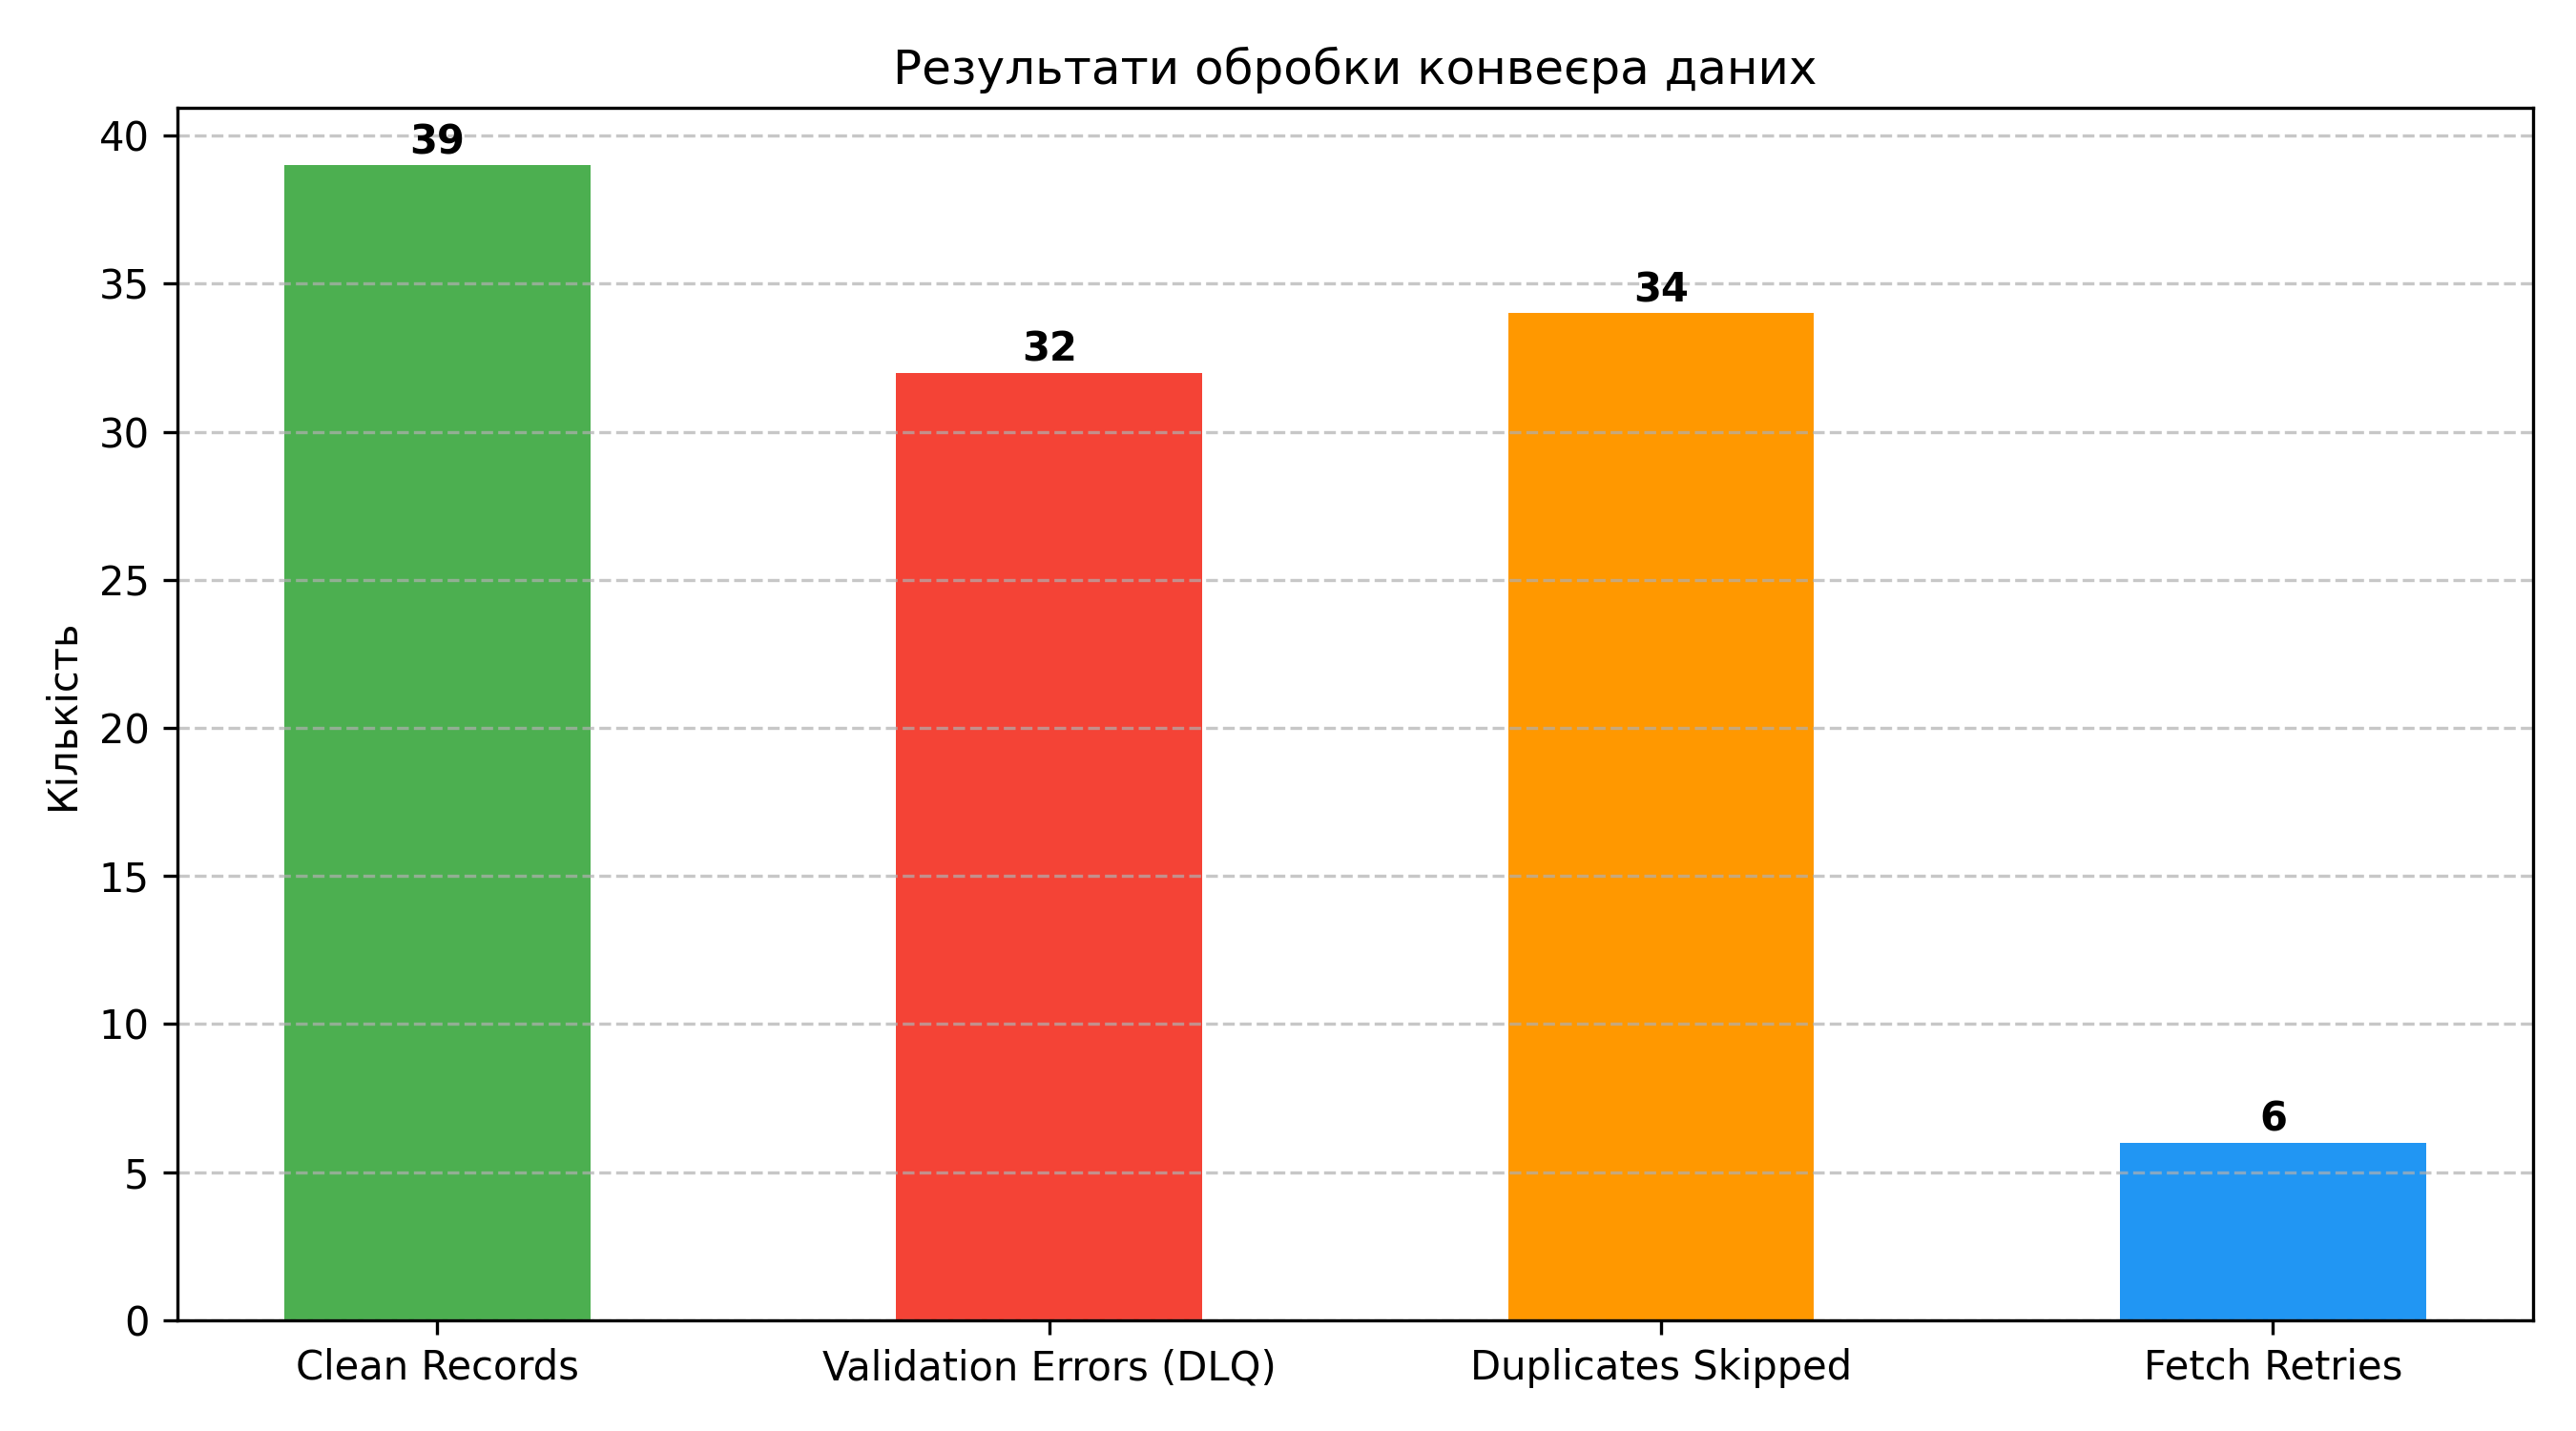
\includegraphics[width=\textwidth]{lab3_metrics.png}
\caption{Розподіл результатів обробки}
\label{fig:metrics}
\end{minipage}
\end{figure}
\end{enumerate}

\rsec{Висновки:} У ході виконання лабораторної роботи №3 побудовано відмовостійкий конвеєр для ненадійних потокових даних датчиків. Генератор вводить пошкоджені записи, дублікати й тимчасові відмови джерела. Конвеєр опрацював усі ці збої: 105 отриманих записів розподілено на 39 чистих, 32 записи в DLQ і 34 пропущені дублікати. Сума збігається з кількістю отриманих, тобто жоден запис не втрачено. Шість тимчасових відмов джерела було подолано повторними спробами з експоненційною затримкою, без жодного втраченого батча. Ідемпотентність на основі \texttt{record\_id}, порядок «дані, потім стан» і атомарний запис файлів гарантують, що повторний запуск або збій посеред обробки не призводять ні до дублікатів, ні до втрати чи пошкодження даних. Dead Letter Queue зберігає некоректні записи разом із причиною відмови, що дає змогу аналізувати якість джерела, а не просто відкидати дані.

\end{document}
